% ── Projekty a úlohy ──────────────────────────────────────────
\chapter{Projekty a úlohy}

        Jadrom aplikácie je správa projektov a~úloh. V~tejto kapitole opisujeme,
ako sme navrhli vytváranie a~organizovanie projektov, priraďovanie úloh
členom tímu a~sledovanie ich stavu od vytvorenia až po dokončenie.

\section{Správa projektov}

        Projekt je základnou organizačnou jednotkou systému. Každý projekt združuje
súvisiace úlohy, dokumenty a~členov tímu. Oprávnený používateľ (administrátor
alebo manažér) môže vytvoriť nový projekt vyplnením formulára s~nasledujúcimi
atribútmi:

\begin{itemize}
  \item \textbf{Názov} -- krátky identifikačný názov projektu
  \item \textbf{Popis} -- podrobnejší opis cieľov a~obsahu projektu
  \item \textbf{Status} -- aktuálny stav projektu (aktívny, dokončený, archivovaný)
\end{itemize}

        Zoznam projektov je zobrazený na prehľadovej stránke s~možnosťou filtrovania
podľa statusu. Každý projekt je zobrazený ako karta s~kľúčovými
informáciami -- názvom, progresom a~poslednou aktualizáciou (obr.~\ref{fig:projekty}).

\begin{figure}[H]
  \centering
  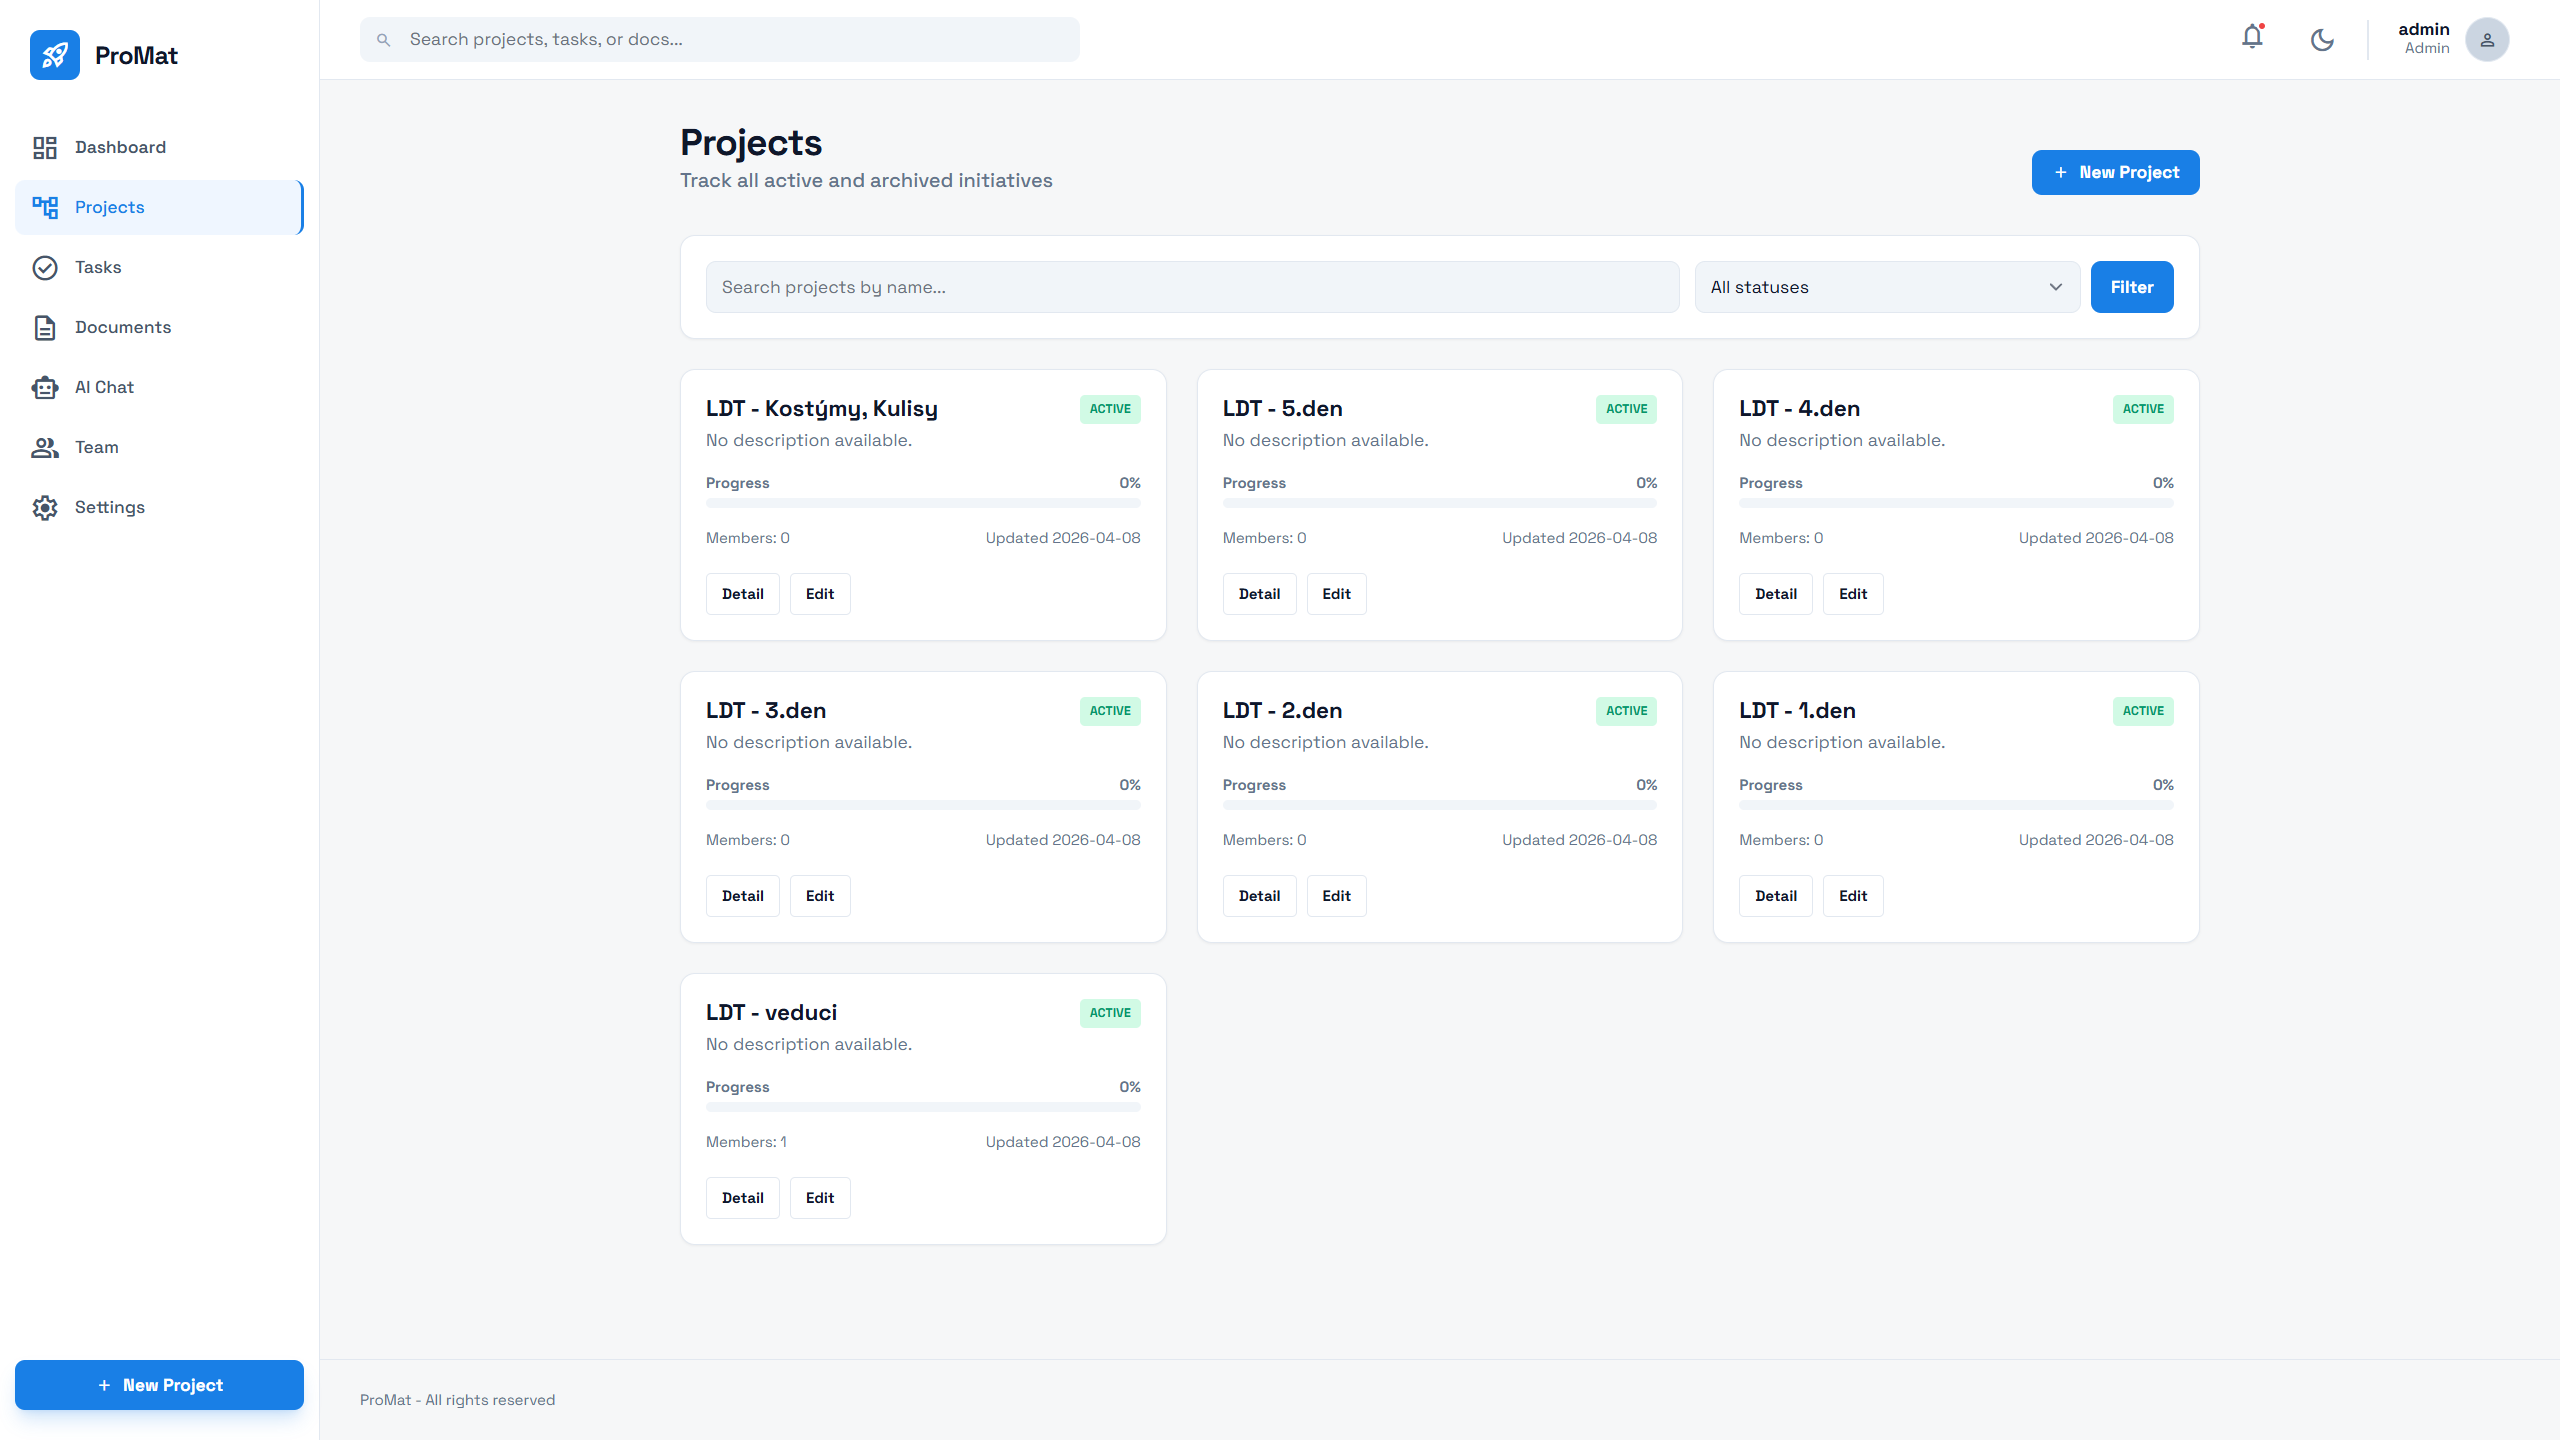
\includegraphics[width=0.9\textwidth]{images/zoznam_projektov.png}
  \caption{Zoznam projektov}
  \label{fig:projekty}
\end{figure}

        Detail projektu zobrazuje všetky úlohy, priradených členov, nahrané dokumenty
a~históriu aktivity (obr.~\ref{fig:detail_projektu}). Projekt je možné upraviť alebo odstrániť len vlastníkovi
alebo administrátorovi.

\begin{figure}[H]
  \centering
  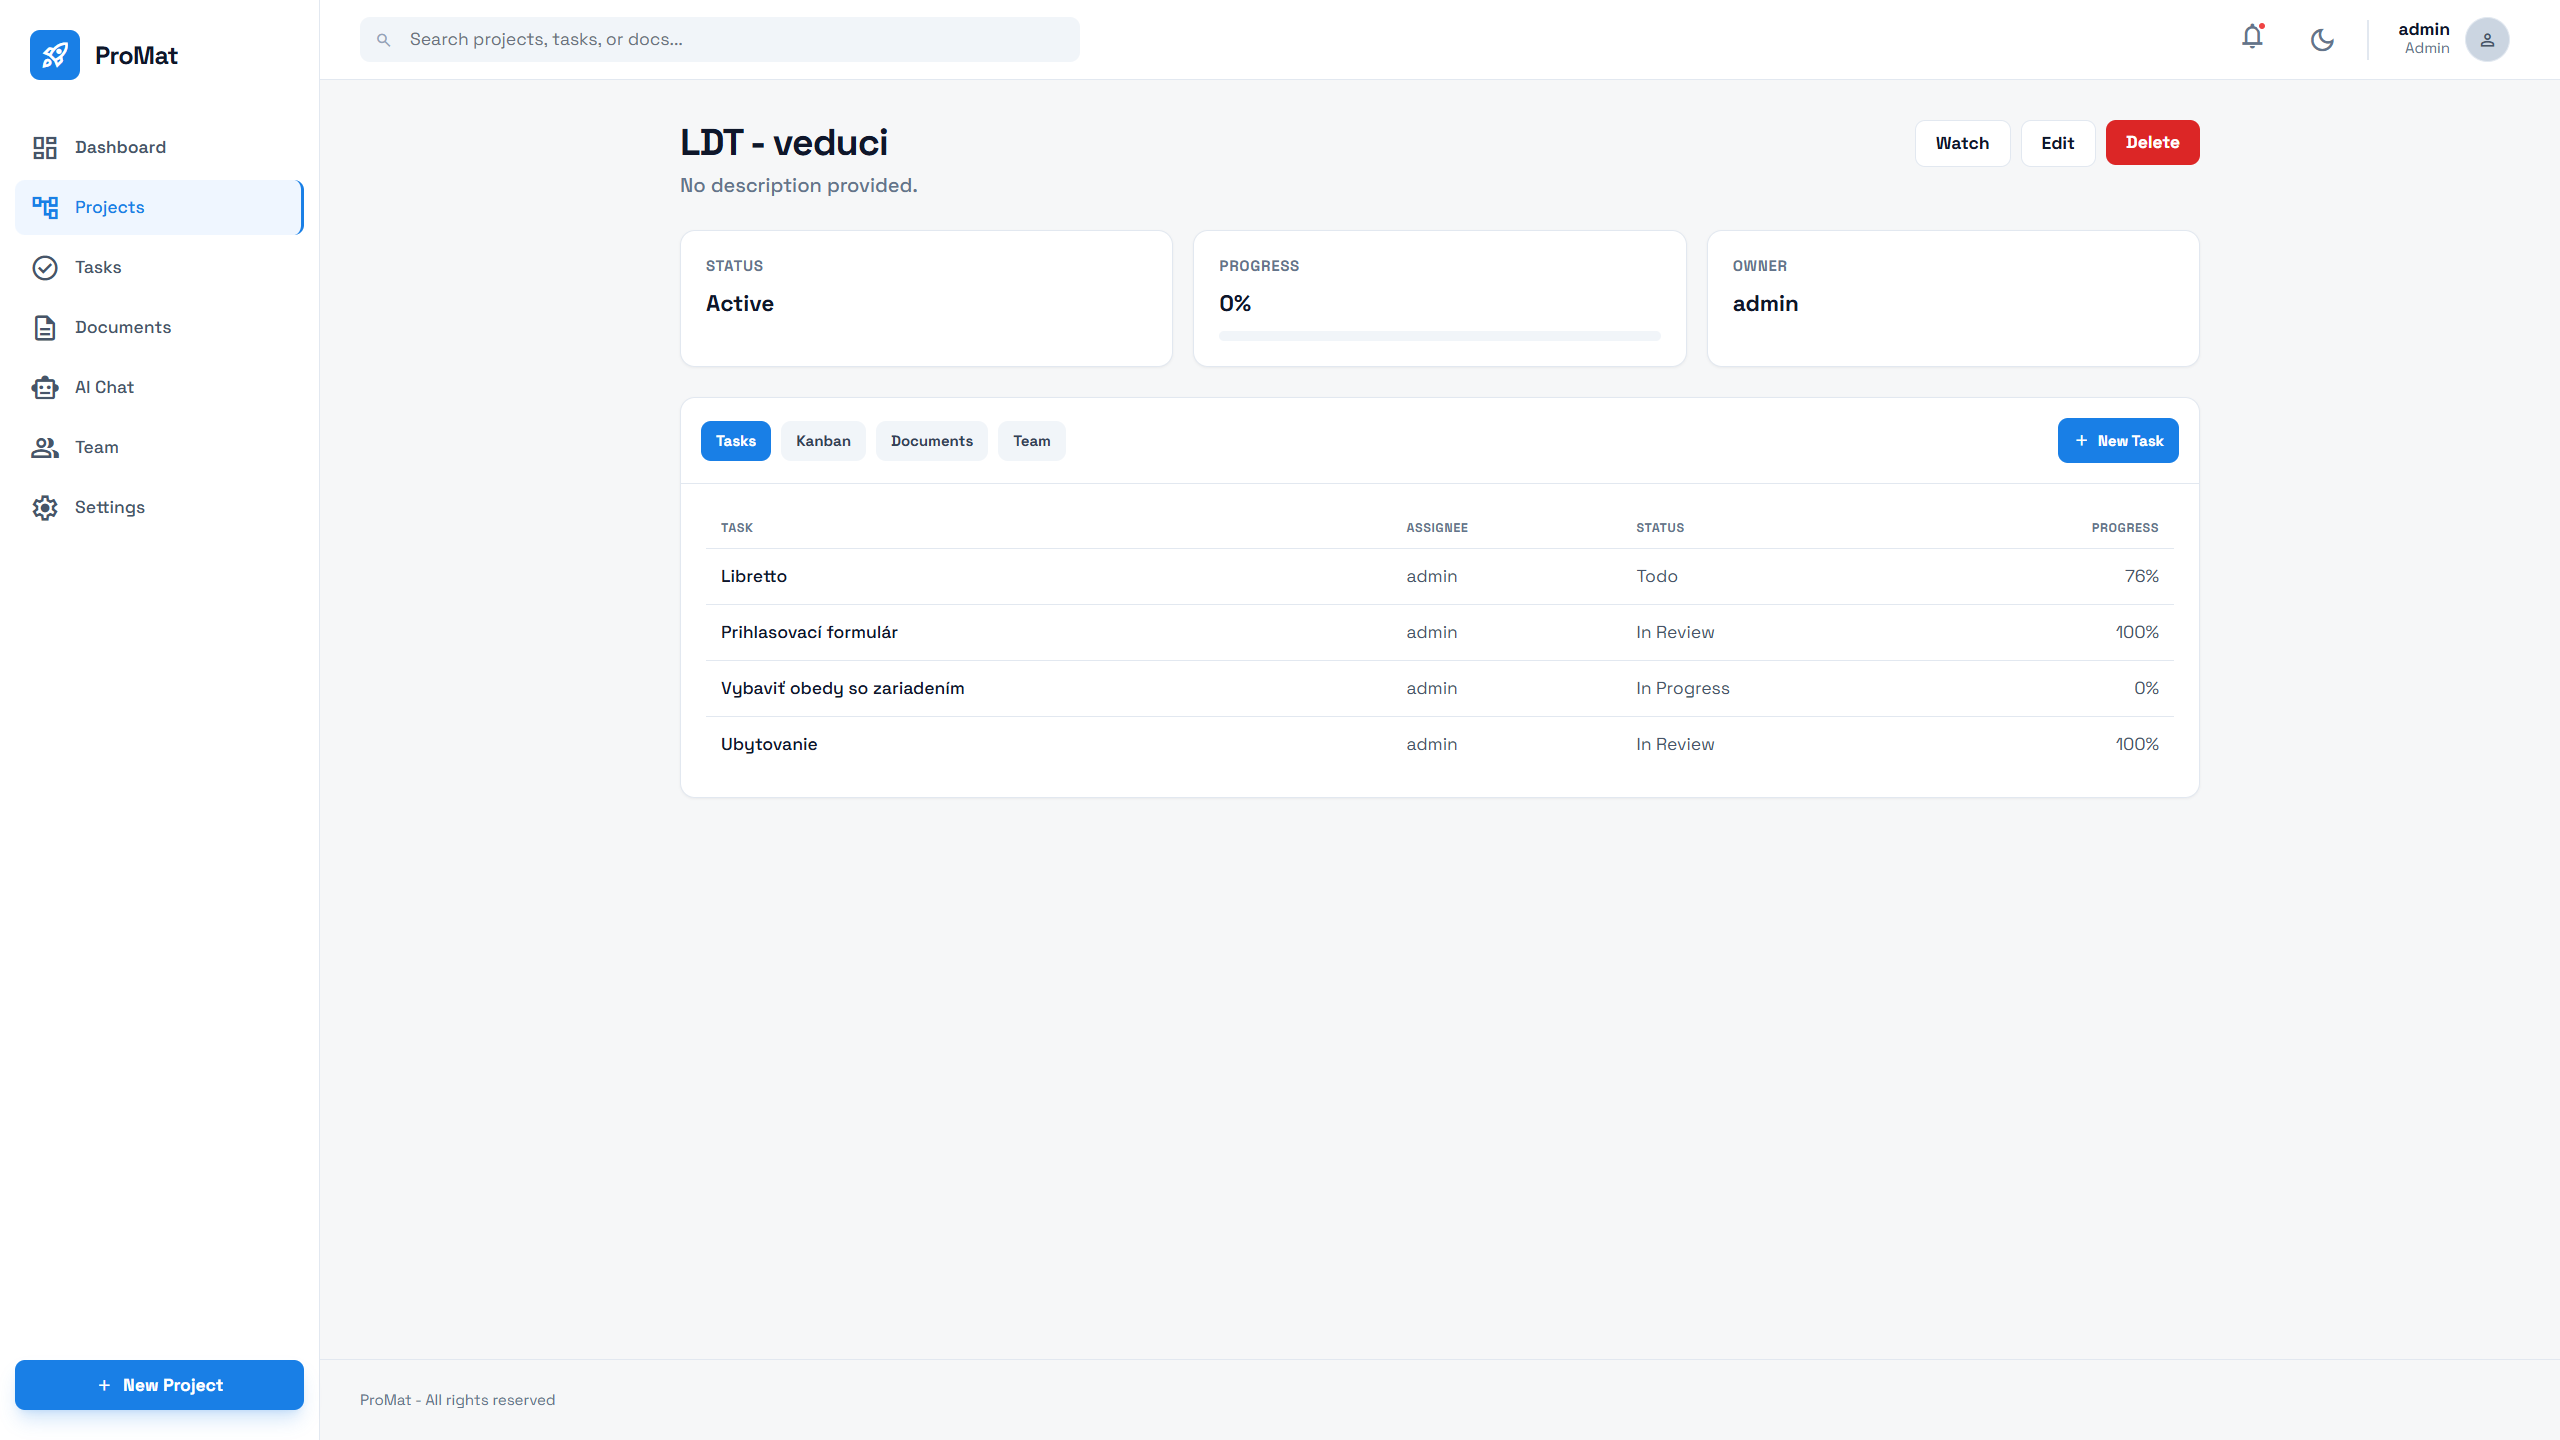
\includegraphics[width=0.9\textwidth]{images/detail_projektu.png}
  \caption{Detail projektu}
  \label{fig:detail_projektu}
\end{figure}

\section{Správa úloh}

        Úlohy sme navrhli ako súčasť konkrétneho projektu. Pri vytváraní úlohy
používateľ zadáva:

\begin{itemize}
  \item \textbf{Názov a~popis} -- čo treba urobiť a~prečo
  \item \textbf{Prioritu} -- nízka, stredná alebo vysoká
  \item \textbf{Termín dokončenia} -- dátum, do ktorého má byť úloha hotová
  \item \textbf{Status} -- aktuálny stav (nová, v~riešení, dokončená)
  \item \textbf{Priradenie} -- člen tímu zodpovedný za splnenie úlohy
\end{itemize}

        Úlohy sú zobrazené vo viacerých pohľadoch. Zoznamový pohľad umožňuje triedenie
a~filtrovanie podľa priority, termínu alebo priradeného člena. Kanban pohľad
zobrazuje úlohy v~stĺpcoch podľa stavu a~umožňuje presúvanie úloh
drag-and-drop interakciou priamo v~prehliadači (obr.~\ref{fig:kanban}).

\begin{figure}[H]
  \centering
  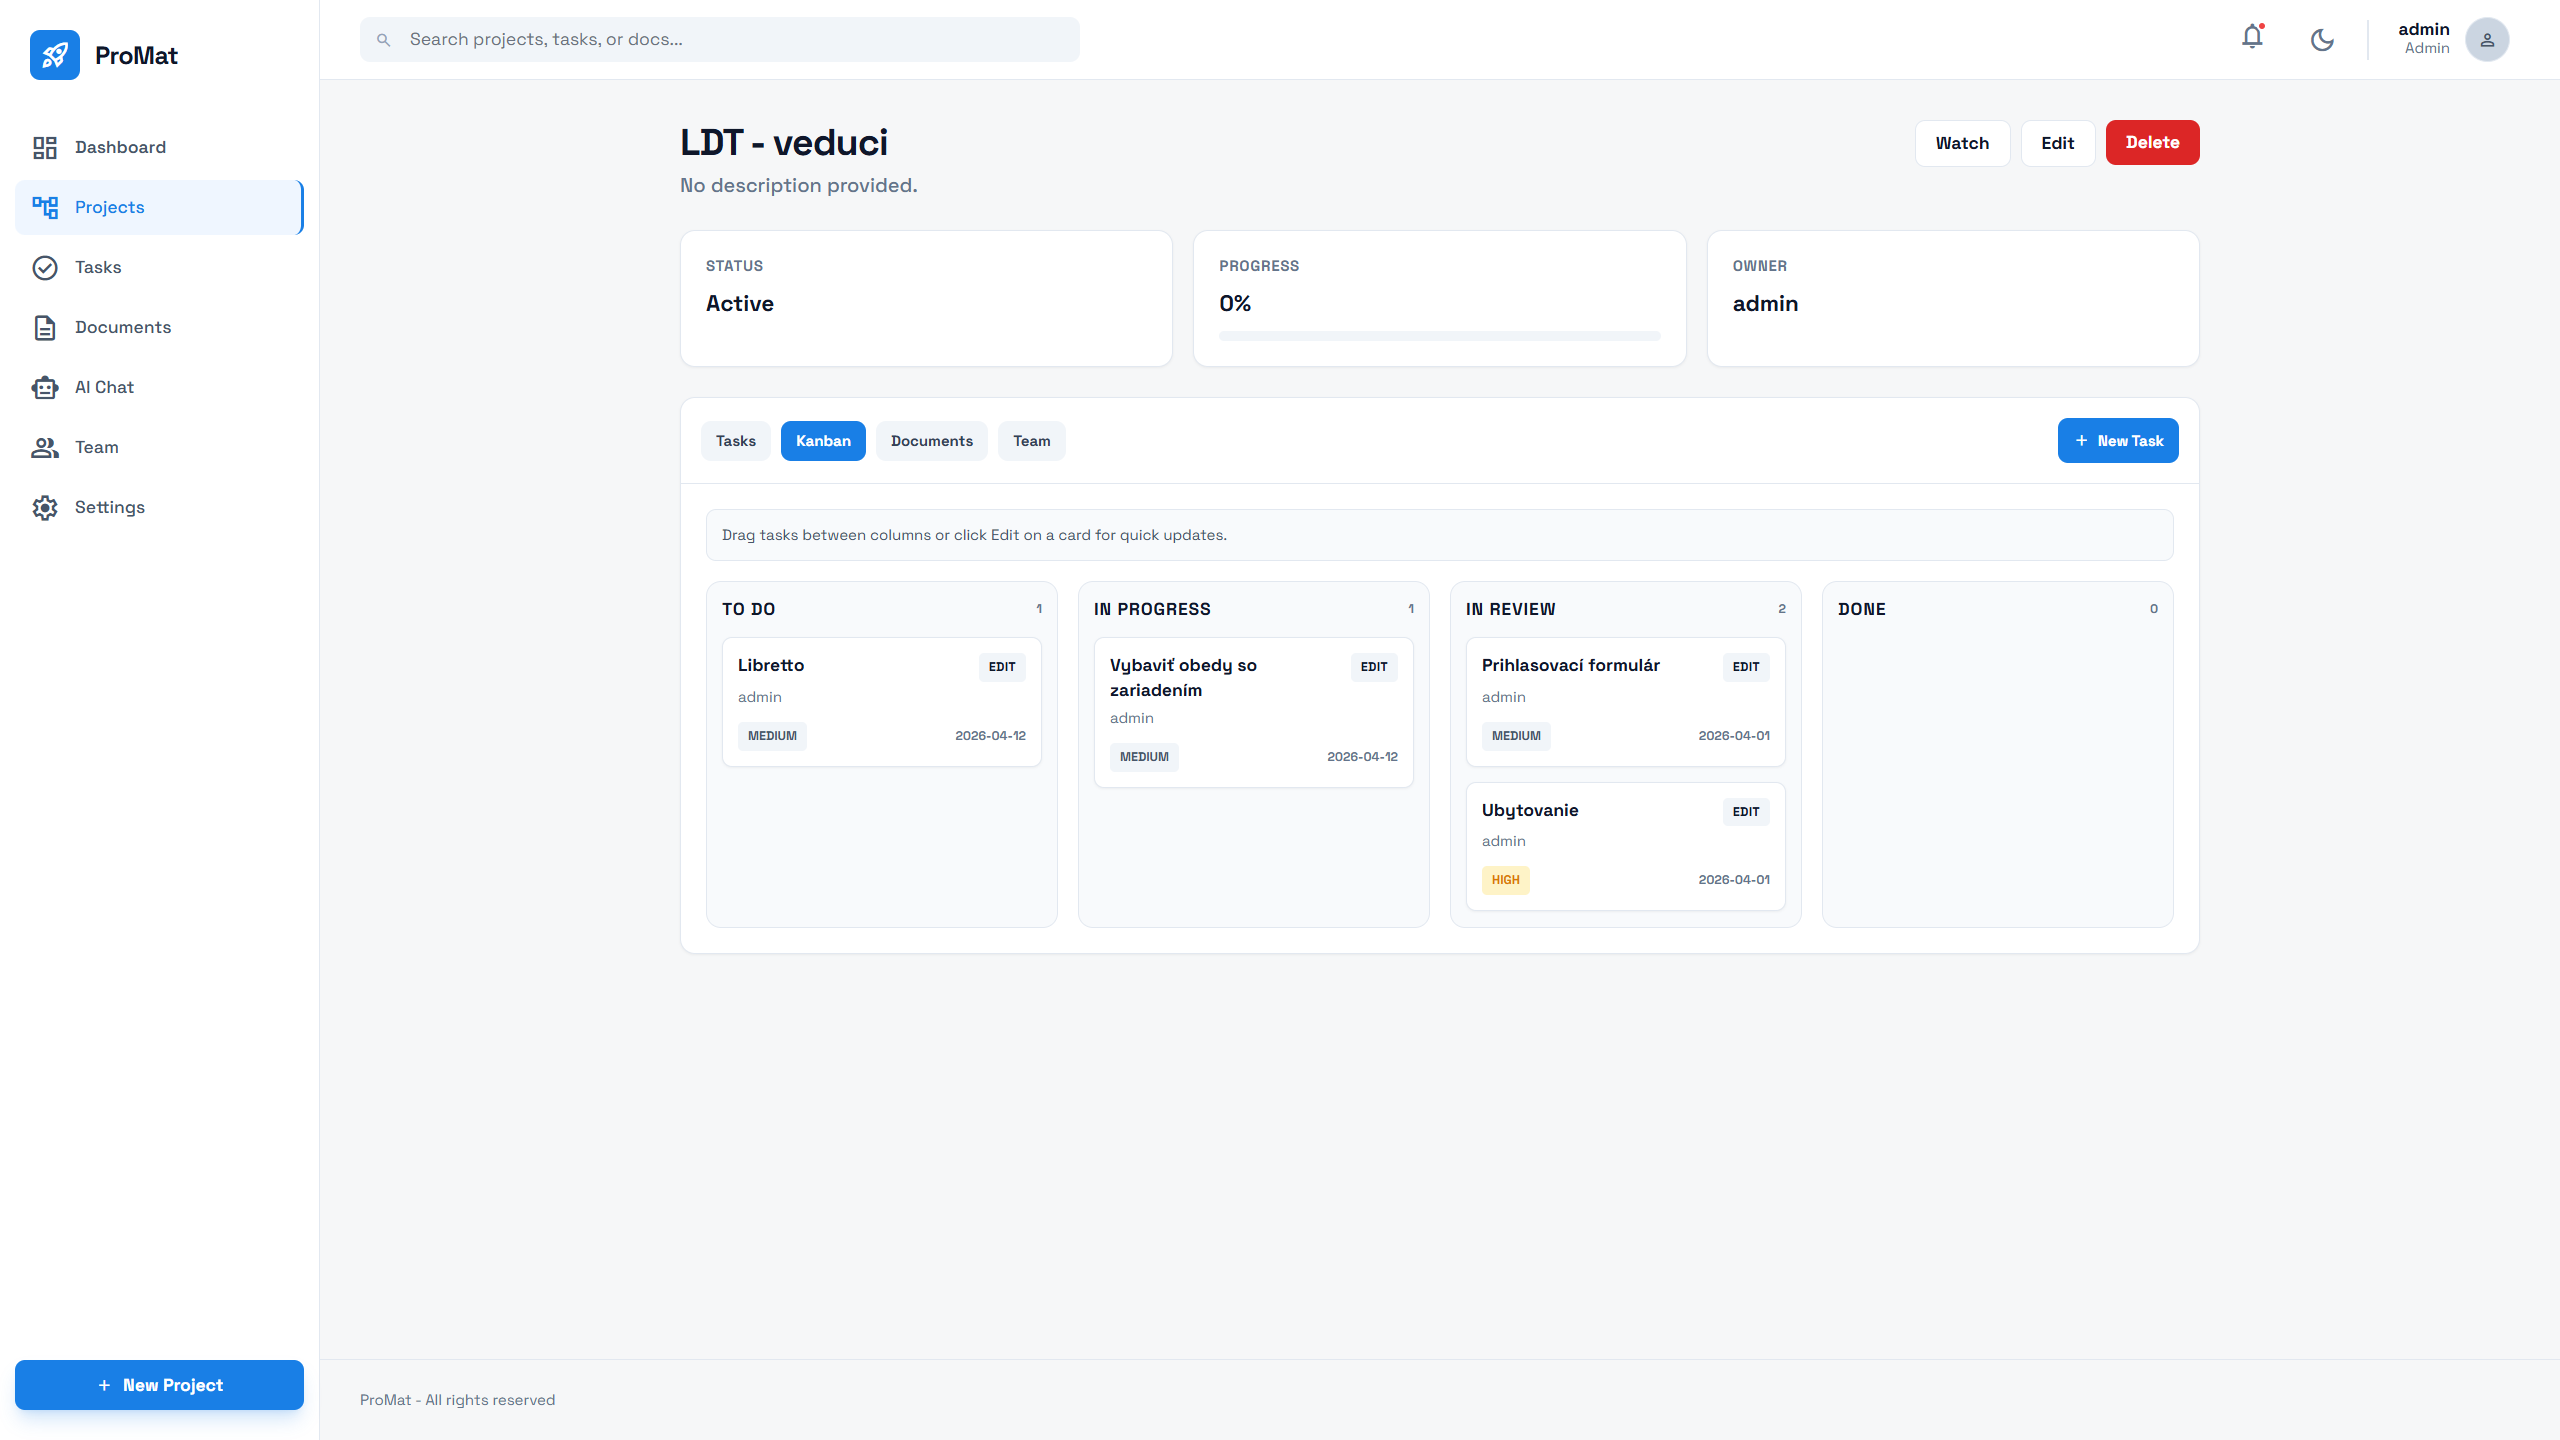
\includegraphics[width=0.9\textwidth]{images/kanban_ulohy.png}
  \caption{Kanban tabuľa úloh projektu}
  \label{fig:kanban}
\end{figure}

        K~úlohe je možné pridávať komentáre, položky na checklist a~prikladať dokumenty. Každá zmena stavu
úlohy generuje upozornenie pre prideleného člena tímu.

\section{Priradenie členov}

        Systém sme navrhli s~podporou viacerých používateľov pracujúcich na jednom projekte.
Administrátor alebo vlastník projektu môže prizvať ďalších registrovaných
používateľov do projektu. Priradení členovia majú prístup k~projektovým úlohám
a~dokumentom v~súlade so svojou systémovou rolou (obr.~\ref{fig:clenovia}).

\begin{figure}[H]
  \centering
  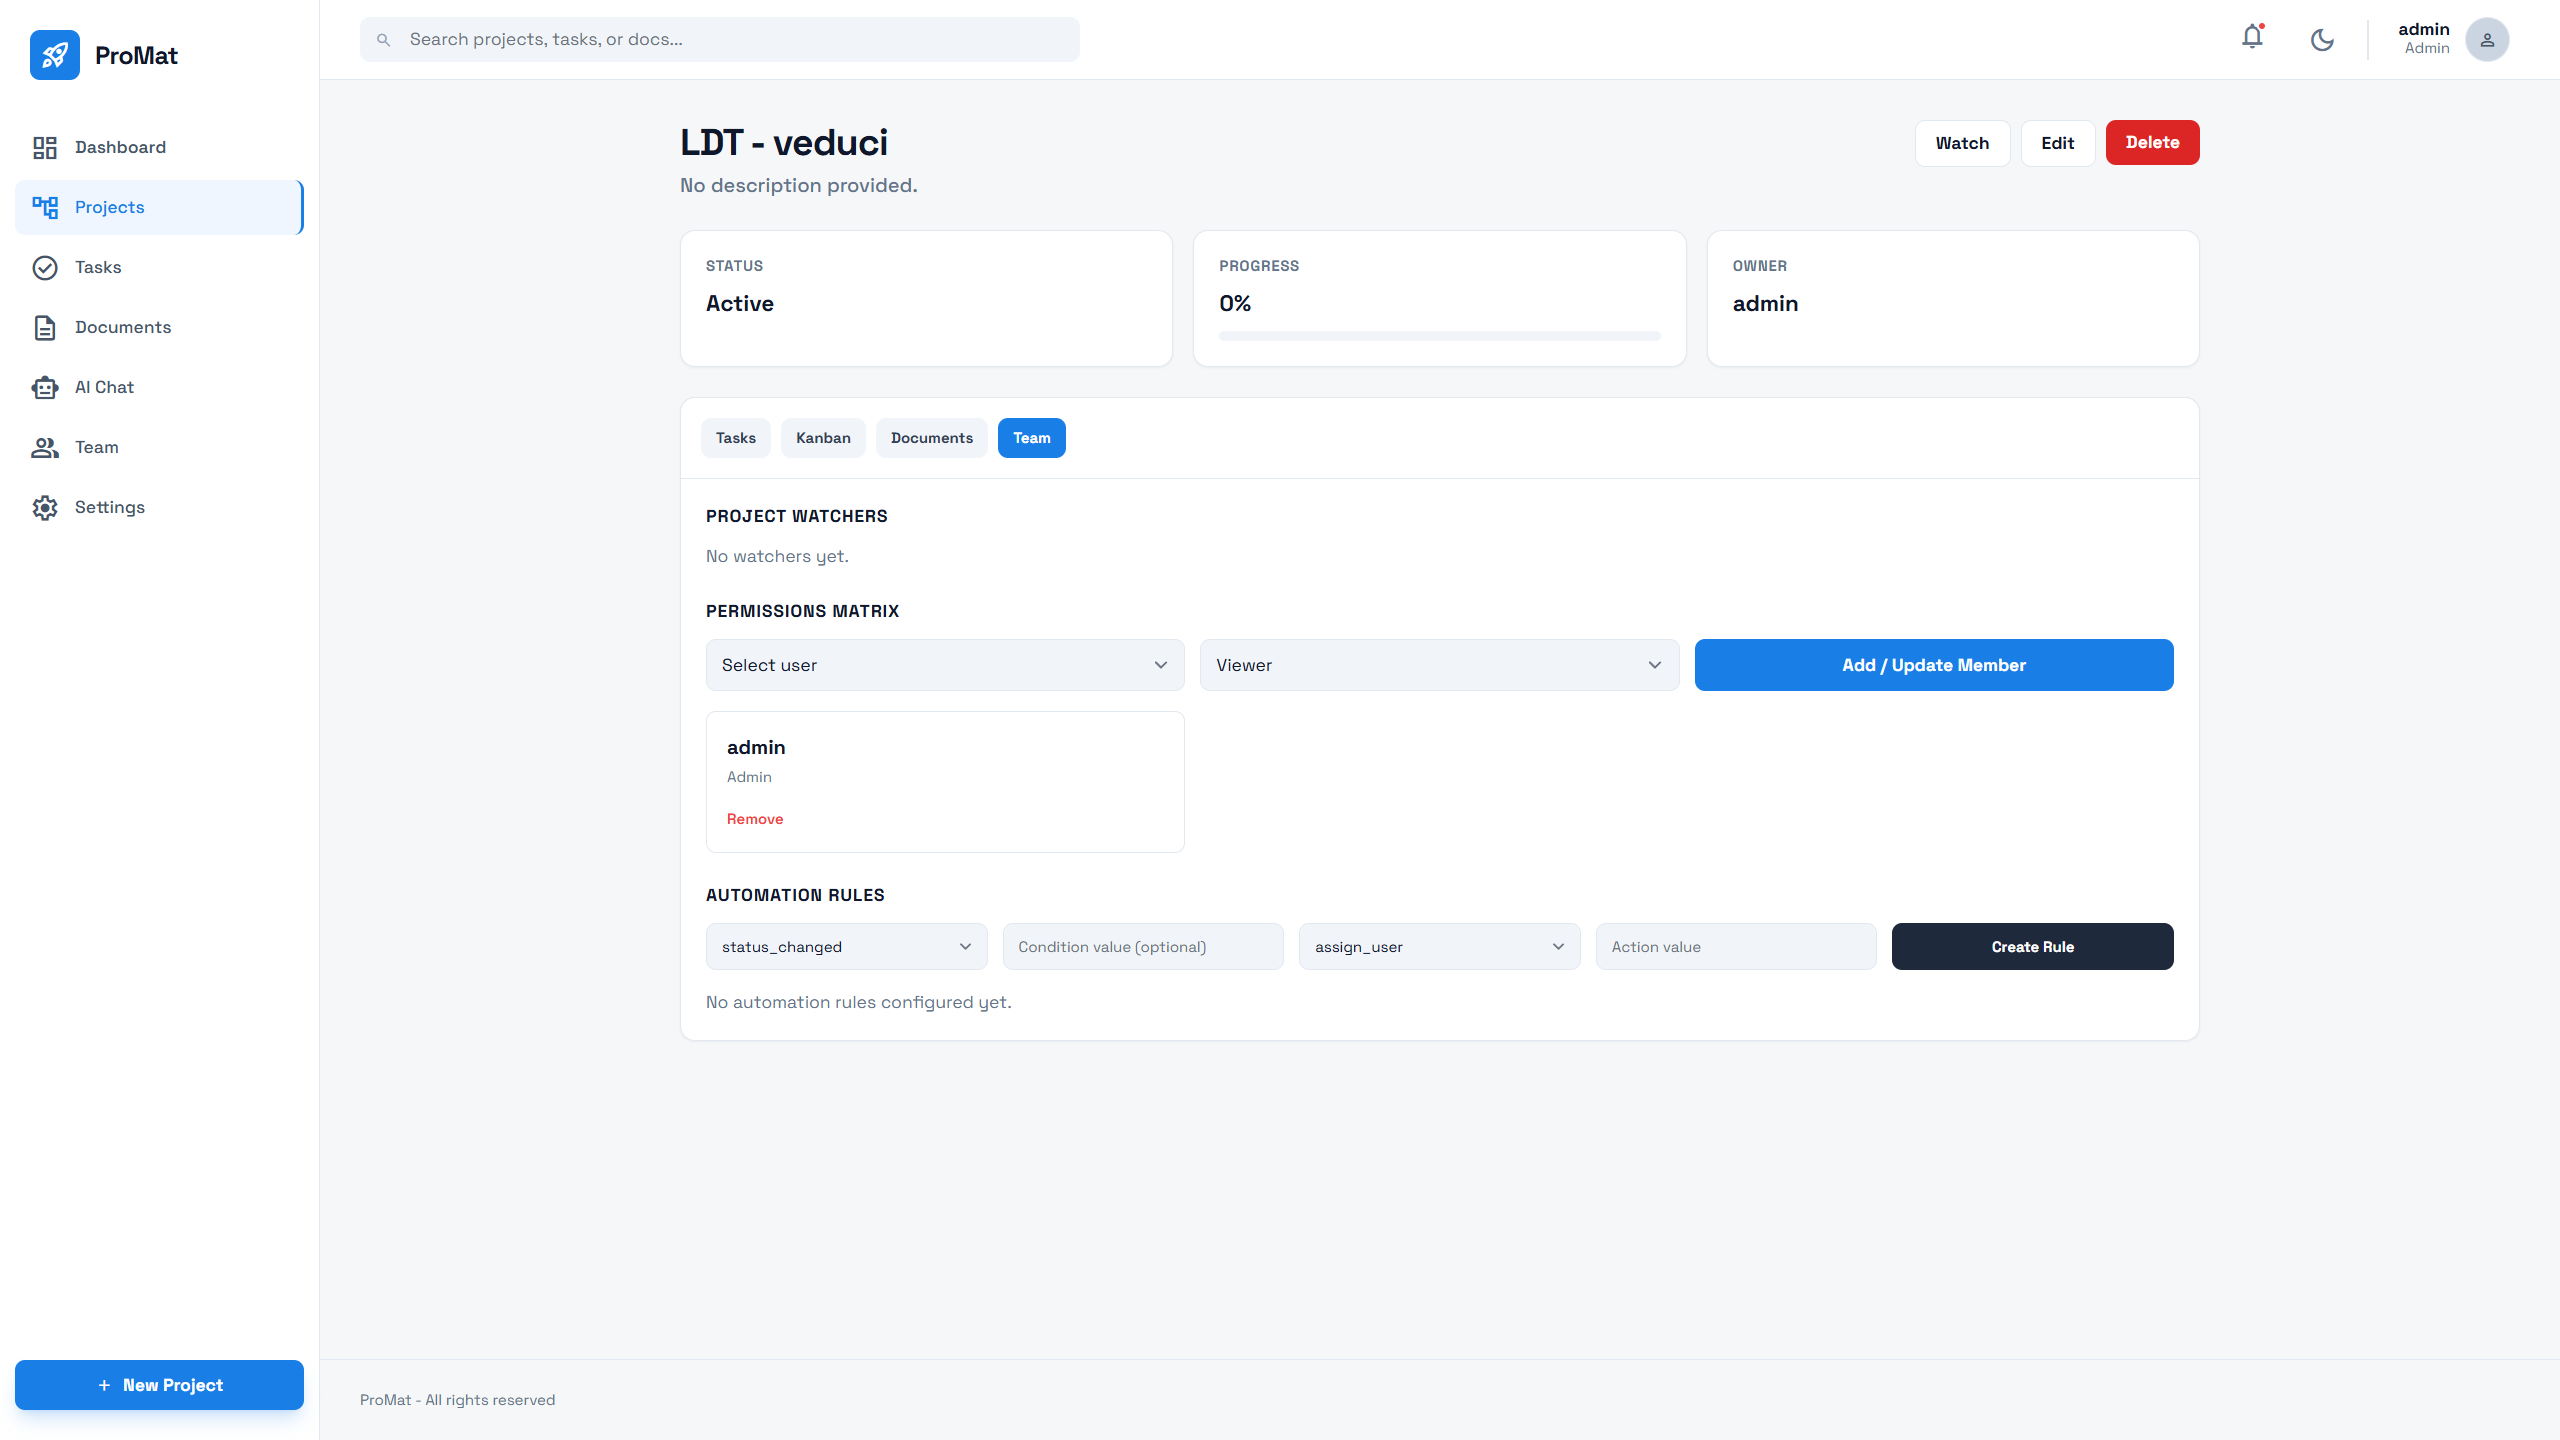
\includegraphics[width=0.85\textwidth]{images/clenovia_projektu.png}
  \caption{Správa členov projektu}
  \label{fig:clenovia}
\end{figure}
